
\section{Prototype / Mockups}

This section presents the Room4U user-interface prototypes and mockups.
The screens illustrate the layout, information hierarchy, navigation,
and main interactions of the system. Room4U provides two role-based
interfaces: the Student Interface and the Administrator Interface. Both
use the Room4U open-book logo and a consistent blue-and-white visual
language, including the account bar, left navigation, room information
panels, status indicators, and primary action buttons. The mockups
communicate the intended appearance and behavior of the system before
implementation.

The following subsections describe the interactive prototypes, screen
list, individual mockups, key confirmation and result dialogs, and
accessibility considerations.

\section*{9.1. Interactive Prototype}\label{interactive-prototype}
\addcontentsline{toc}{section}{9.1. Interactive Prototype}

Room4U provides separate navigation flows for Student and Administrator
roles. The Student prototype covers room discovery, availability
checking, booking submission, request tracking, request details,
cancellation, history, and logout. The Administrator prototype covers
request processing, room management, room creation and editing, room
suspension and resumption, room-usage schedules, and maintenance
scheduling.

\begin{itemize}
\item
  Student Interactive Prototype: Students can search for meeting rooms,
  inspect room information and availability, submit booking requests,
  review request statuses and details, cancel eligible requests, view
  processed requests, and log out.

  \begin{itemize}
  \item
    \textbf{Prototype Link:}
    \href{https://www.figma.com/proto/0kLDFGO5txhnNfoH99CaKa/Room4U---Version-3?node-id=7-4}{Figma Student Prototype}
  \end{itemize}
\item
  Administrator Interactive Prototype: Administrators can review and
  process booking requests, approve or reject pending requests, cancel
  approved bookings when permitted, manage room information, suspend or
  resume rooms, inspect room usage, and create or remove maintenance
  schedules. The interface also provides confirmation, success, and
  validation dialogs for important actions.

  \begin{itemize}
  \item
    \textbf{Prototype Link:}
    \href{https://www.figma.com/proto/0kLDFGO5txhnNfoH99CaKa/Room4U---Version-3?node-id=51-239}{Figma Administrator Prototype}
  \end{itemize}
\end{itemize}

\section*{9.2. Screen List and Mockups}\label{screen-list-and-mockups}
\addcontentsline{toc}{section}{9.2. Screen List and Mockups}

This subsection lists the main Room4U screens and their associated use
cases. The screens are grouped by user role. Each entry identifies the
screen's purpose and summarizes the information,
actions, and important interaction states represented by the mockups.

\subsection*{Screen List}
\addcontentsline{toc}{subsection}{Screen List}
\label{screen-list}

\begin{longtable}{|p{0.16\textwidth}|p{0.39\textwidth}|p{0.35\textwidth}|}
\hline
\textbf{Screen ID} & \textbf{Screen Name} & \textbf{Related Use Case(s)} \\
\hline
\endfirsthead
\hline
\textbf{Screen ID} & \textbf{Screen Name} & \textbf{Related Use Case(s)} \\
\hline
\endhead
S01 & Sign In & UC-01 \\
\hline
S02 & Room Search and Availability & UC-02, UC-03 \\
\hline
S03 & Booking Request & UC-04 \\
\hline
S04 & My Requests, Details and History & UC-02, UC-05, UC-06 \\
\hline
S05 & Admin Request Queue & UC-02, UC-07 \\
\hline
S06 & Request Details and Processing & UC-07, UC-08, UC-09, UC-10 \\
\hline
S07 & Room Management & UC-11, UC-12 \\
\hline
S08 & Room Availability and Maintenance & UC-13 \\
\hline
\end{longtable}

\section*{9.2.1. Student Interface}\label{student-interface}
\addcontentsline{toc}{section}{9.2.1. Student Interface}

The Student Interface supports the complete student-side booking flow.
Students can sign in, search for rooms, inspect availability, submit a
booking request, monitor its status, open request details, cancel an
eligible request, review request history, and log out.

\subsection*{9.2.1.1. S01 - Sign In}\label{s01---sign-in}
\addcontentsline{toc}{subsection}{9.2.1.1. S01 - Sign In}

\begin{itemize}
\item
  Description: This screen is the entry point for both Student and
  Administrator users. It provides Email and Password fields and a Sign
  In button. Users sign in with accounts provided by the system; no
  public registration flow is shown. The screen includes Room4U branding
  and a short explanation of the service. If authentication fails, an
  error message is displayed so the user can check the credentials and
  try again.
\item
  \textbf{Mockup View:}
\end{itemize}

\begin{quote}
\begin{center}
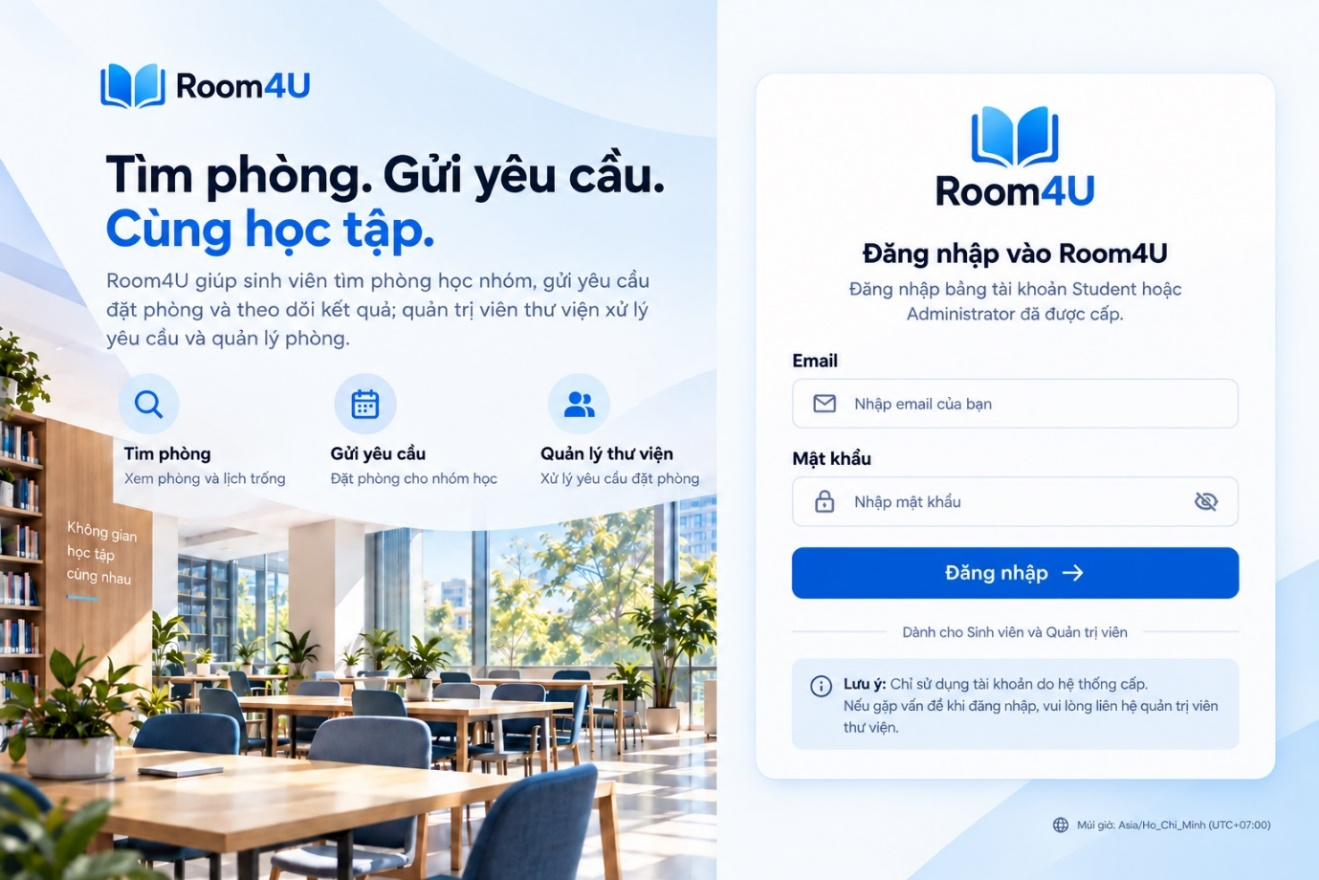
\includegraphics[width=0.9\textwidth,height=0.72\textheight,keepaspectratio]{images/image1.jpeg}
\end{center}
\end{quote}

\subsection*{9.2.1.2. S02 - Room Search and
Availability}\label{s02---room-search-and-availability}
\addcontentsline{toc}{subsection}{9.2.1.2. S02 - Room Search and
Availability}

\begin{itemize}
\item
  Description: This flow helps students find a suitable meeting room and
  check its schedule before submitting a booking request. It consists of
  room-search results and a room-availability view.

  \begin{itemize}
  \item
    Room Search: Students can search using available criteria such as
    the intended date, number of people, and room requirements. Results
    are presented as room cards showing a room image, room name,
    capacity, floor, equipment, current status, and an action to inspect
    the room or its availability.
  \item
    Room Availability: After selecting a room, students can view its
    time-slot schedule for a selected date. The schedule distinguishes
    available periods from approved bookings, maintenance periods, and
    other unavailable periods so that students can choose a valid time
    before opening the booking-request form.
  \end{itemize}
\item
  \textbf{Mockup Views:}
\end{itemize}

\subsubsection*{S02.1 -- Room Search}
\addcontentsline{toc}{subsubsection}{S02.1 -- Room Search}

\begin{center}
\begin{center}
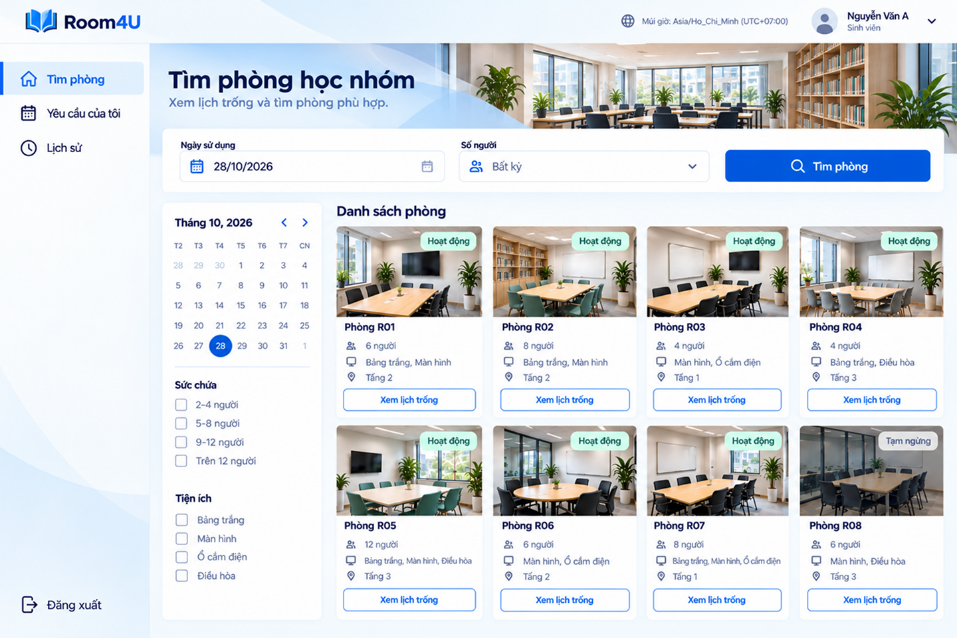
\includegraphics[width=0.9\textwidth,height=0.72\textheight,keepaspectratio]{images/image2.png}
\end{center}
\end{center}

\subsubsection{S02.2 -- Room
Availability}\label{s02.2-room-availability}

\begin{quote}
\begin{center}
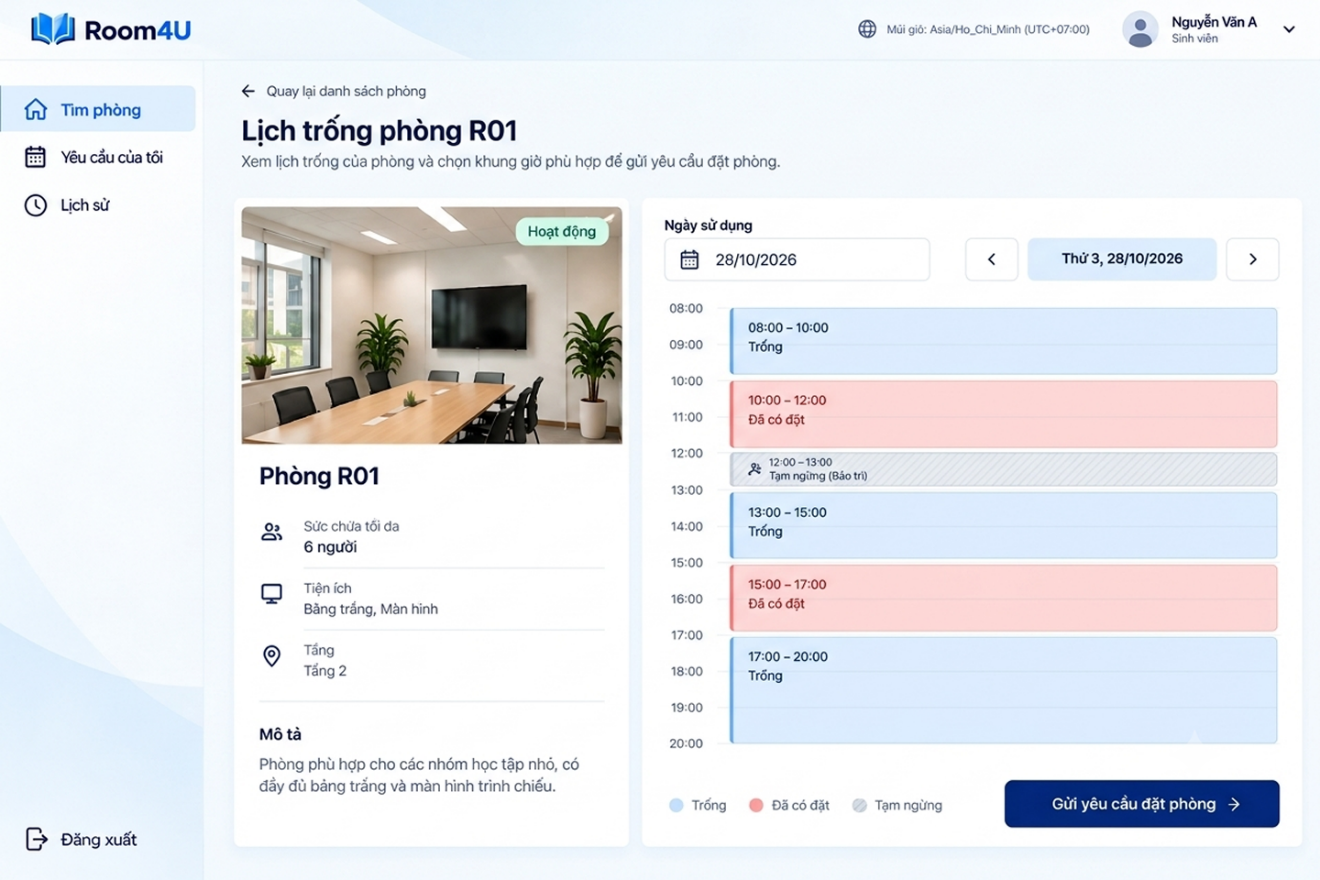
\includegraphics[width=0.9\textwidth,height=0.72\textheight,keepaspectratio]{images/image3.png}
\end{center}
\end{quote}

\subsection*{9.2.1.3. S03 - Booking
Request}\label{s03---booking-request}
\addcontentsline{toc}{subsection}{9.2.1.3. S03 - Booking Request}

\begin{itemize}
\item
  Description: This screen allows a student to submit a booking request
  for the selected room. The form displays the room information and
  collects the usage date, start time, duration, number of participants,
  purpose of use, and an optional note. The available duration options
  are 30, 60, 90, and 120 minutes. The system calculates the end time
  from the selected start time and duration and displays it for the
  student to review. The start time must be later than the current time
  and no more than seven days from the current time (BR-04). The system
  validates the request against room capacity, availability, and the
  applicable booking rules. A successfully submitted request receives a
  request ID and appears with Pending status in the
  student's request list.
\item
  \textbf{Mockup View:}
\end{itemize}

\begin{center}
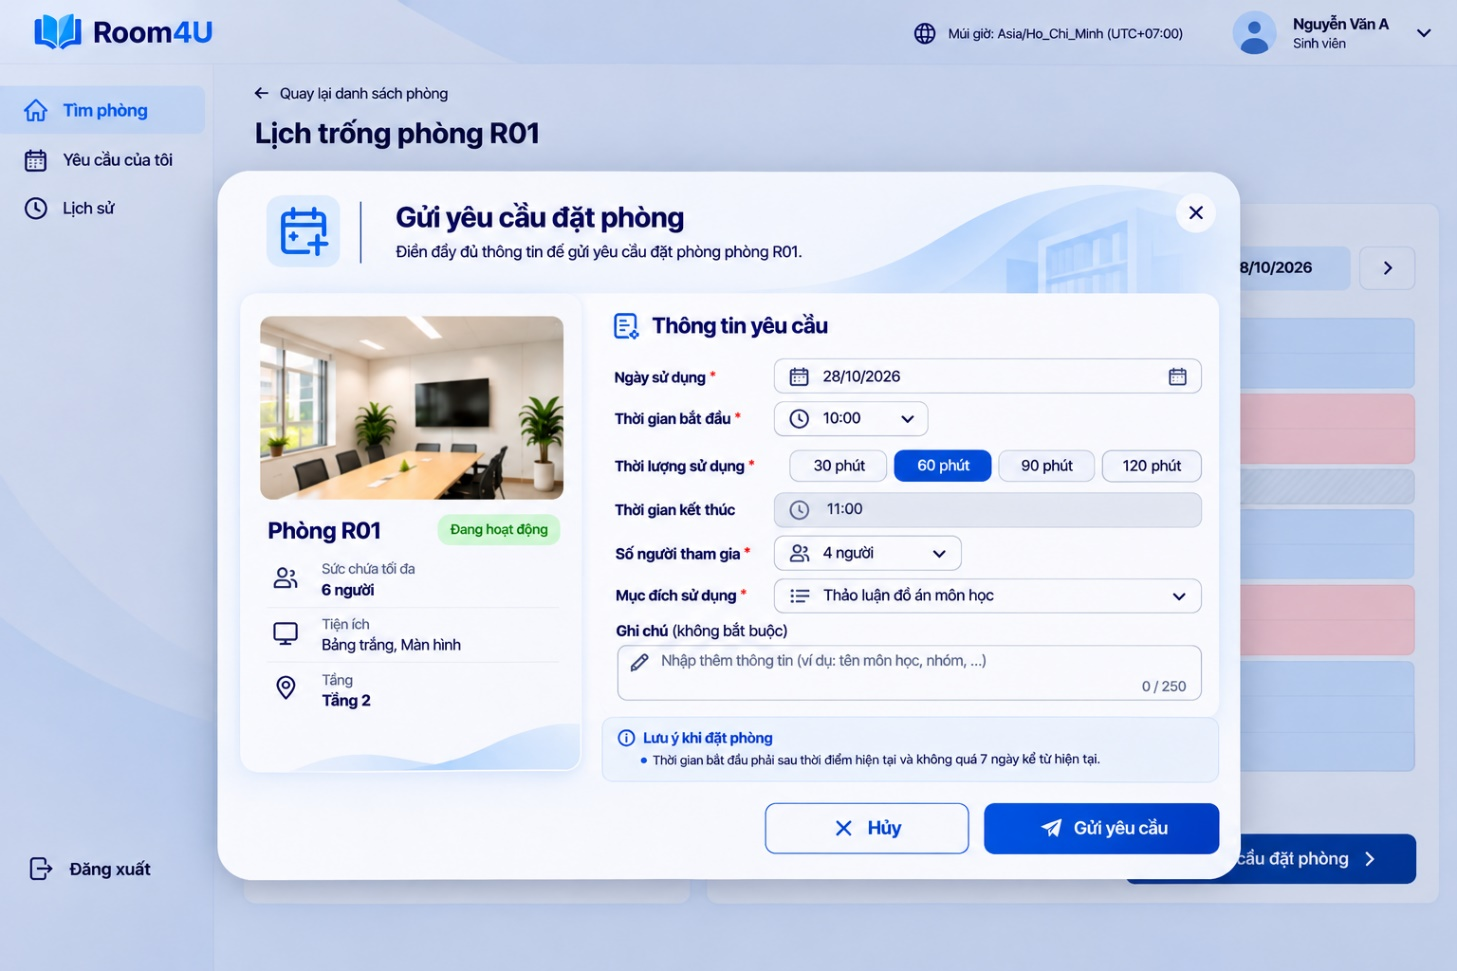
\includegraphics[width=0.9\textwidth,height=0.72\textheight,keepaspectratio]{images/image4.jpeg}
\end{center}

\begin{center}
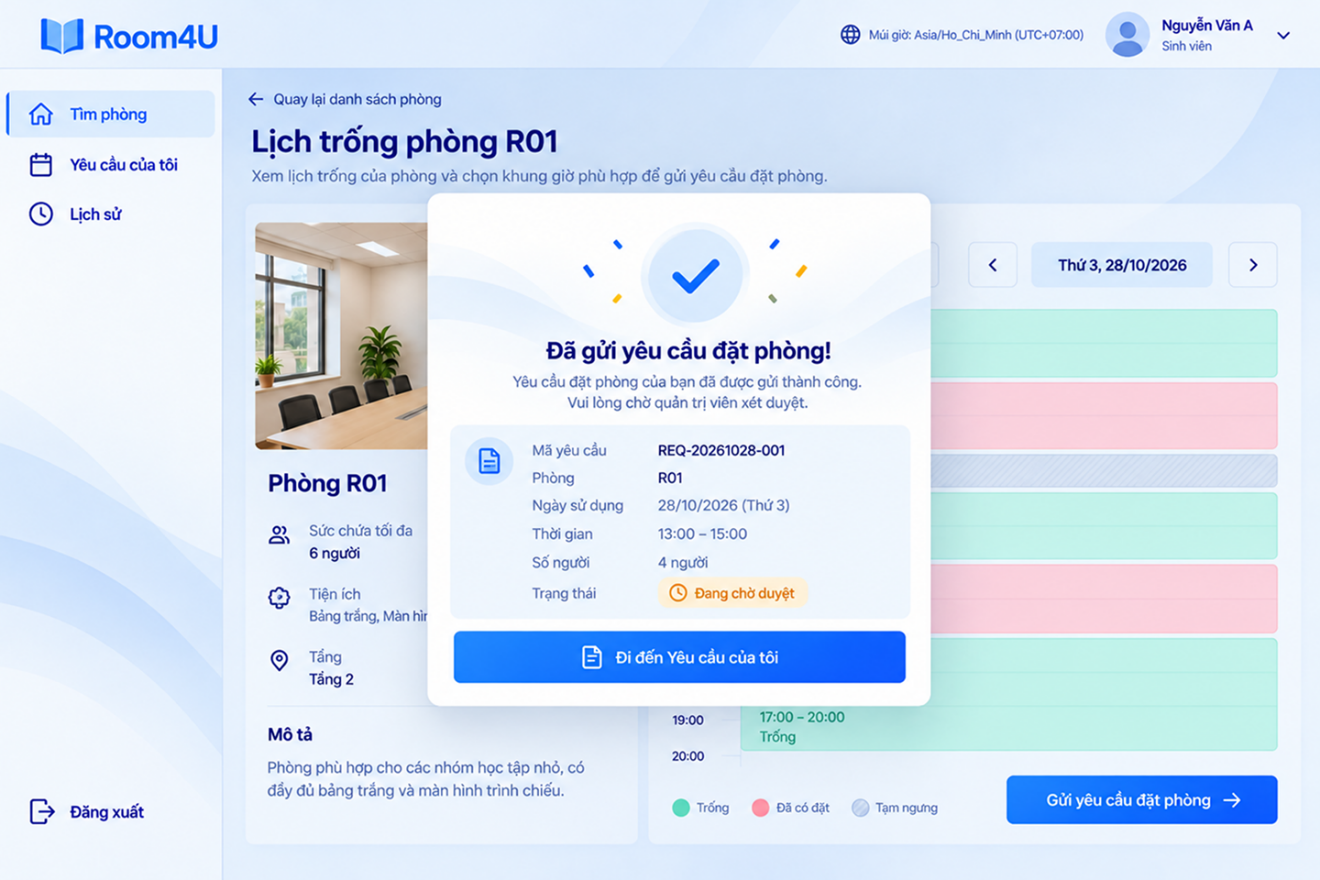
\includegraphics[width=0.9\textwidth,height=0.72\textheight,keepaspectratio]{images/image5.png}
\end{center}

\subsection*{9.2.1.4. S04 - My Requests and
History}\label{s04---my-requests-and-history}
\addcontentsline{toc}{subsection}{9.2.1.4. S04 - My Requests and
History}

\begin{itemize}
\item
  Description: This area allows students to monitor submitted booking
  requests and review requests that have already been processed. The
  active-request screen provides search and status filters. Each row
  shows the request ID, room, usage date and time, purpose, current
  status, and a View Details action. Students can open a request to
  inspect its full information. A separate History screen lists
  previously processed requests.
\end{itemize}

\subsection*{9.2.1.4.1. S04.1 - My Requests
List}\label{s04.1---my-requests-list}
\addcontentsline{toc}{subsection}{9.2.1.4.1. S04.1 - My Requests List}

This screen displays the student's request list. Status
tabs help students narrow the results, while the search field supports
searching by request ID, room, or purpose. The table presents the
request ID, room, usage date and time, purpose, status, and a View
Details action. Pagination is provided when the results exceed one page.

\begin{itemize}
\item
  \textbf{Mockup View :}
\end{itemize}

\begin{center}
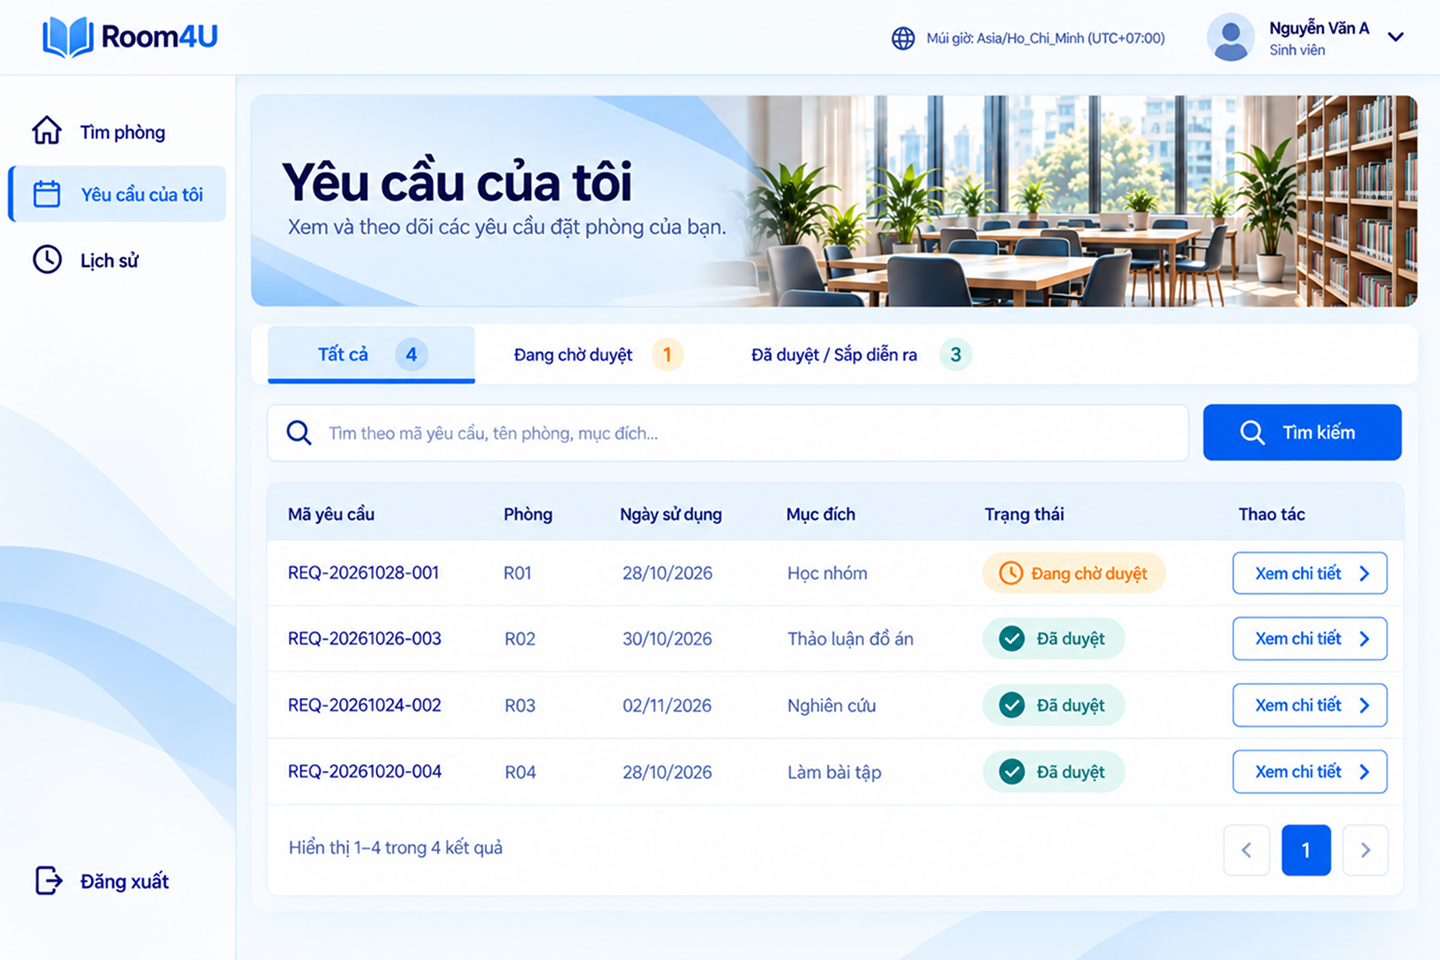
\includegraphics[width=0.9\textwidth,height=0.72\textheight,keepaspectratio]{images/image6.png}
\end{center}

\subsection*{9.2.1.4.2. S04.2 - Booking Request
Details}\label{s04.2---booking-request-details}
\addcontentsline{toc}{subsection}{9.2.1.4.2. S04.2 - Booking Request
Details}

This screen presents the full information for one selected request. It
includes the request ID and current status, room information, usage date
and time, number of participants, purpose, optional note, and requester
information. The student can use Cancel Request when cancellation is
permitted. Cancellation is subject to the applicable request-status and
booking-time rules; it is not an unconditional action.

\begin{itemize}
\item
  \textbf{Mockup View:}
\end{itemize}

\begin{quote}
\begin{center}
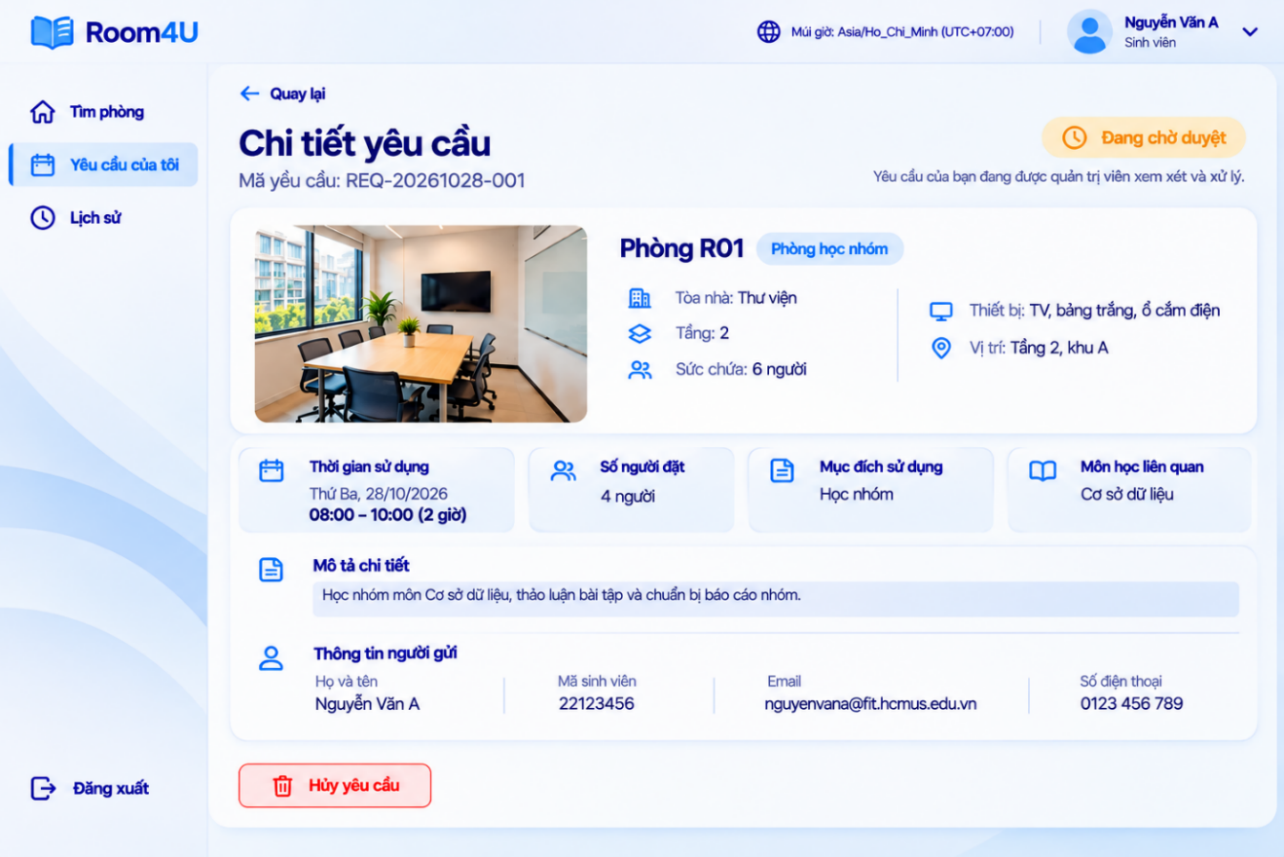
\includegraphics[width=0.9\textwidth,height=0.72\textheight,keepaspectratio]{images/image7.png}
\end{center}
\end{quote}

Cancellation Interaction: When a student selects Cancel Request for an
eligible request, the system asks for confirmation before changing the
request status. If cancellation is not allowed, the interface explains
why the action cannot proceed. Closing the dialog or choosing not to
continue leaves the request unchanged.

History Function: The History screen allows students to review
previously processed booking requests. It includes Rejected and
Cancelled requests, as well as Approved requests whose scheduled usage
time has passed. An approved request retains its Approved status; the
interface may indicate that its scheduled time has passed rather than
changing the status to Completed. The history table shows the request
ID, room, usage date, purpose, status, and a View Details action. Search
and pagination help students locate older records.

Logout Interaction: The Logout option is available in the left
navigation. Selecting it opens a confirmation dialog over the current
page. The dialog provides Cancel and Log Out actions. Cancel closes the
dialog and keeps the student on the current page; Log Out ends the
session and returns the user to the Sign In screen.

\begin{itemize}
\item
  Mockup View -- History Page with Logout Confirmation:
\end{itemize}

\begin{center}
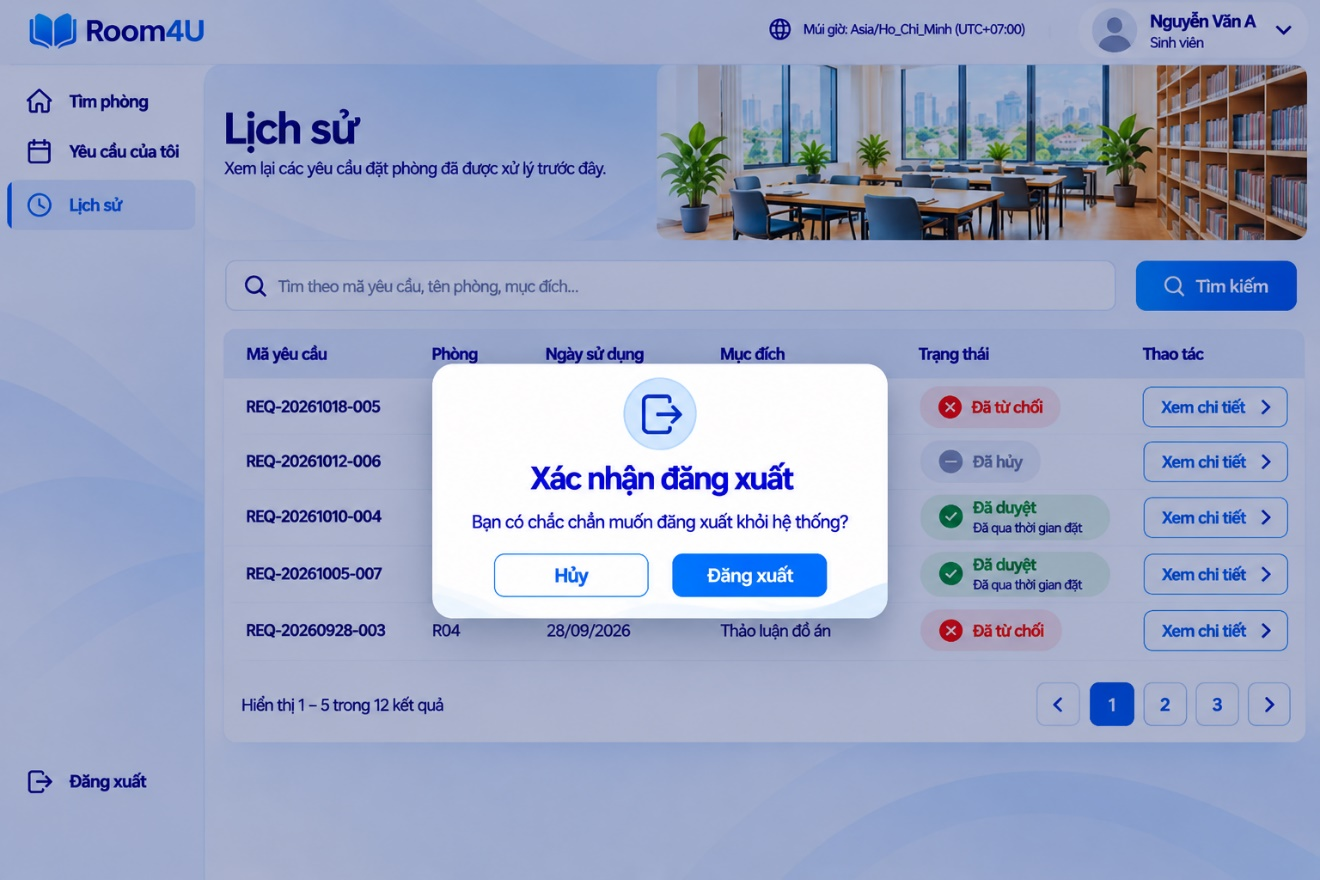
\includegraphics[width=0.9\textwidth,height=0.72\textheight,keepaspectratio]{images/image8.jpeg}
\end{center}

\section*{9.2.2. Administrator Interface}\label{administrator-interface}
\addcontentsline{toc}{section}{9.2.2. Administrator Interface}

The Administrator Interface supports the management and supervision of
Room4U operations. Administrators can review and process student booking
requests, inspect request details and processing history, approve or
reject pending requests, and cancel approved bookings when the
applicable conditions are met. The interface also provides
room-management functions, including adding rooms, updating room
information, and suspending or resuming rooms. In addition,
administrators can monitor room usage, view maintenance schedules,
create maintenance blocks, and remove the effect of eligible future
maintenance blocks while retaining their records. Confirmation, success,
and error dialogs provide feedback for important actions and prevent
changes when the required conditions are not satisfied.

\subsection*{9.2.2.1. S05 - Admin
Dashboard}\label{s05---admin-dashboard}
\addcontentsline{toc}{subsection}{9.2.2.1. S05 - Admin Dashboard}

\begin{itemize}
\item
  Description: This screen is the administrator' s
  request-management queue. It provides status categories for Pending,
  Approved, Rejected, and Cancelled requests, together with a search
  field and a submission-date filter. The request table displays key
  information such as request ID, room, requested usage period, number
  of participants, submission time, and current status. Administrators
  select View Details to inspect and process an individual request.
\item
  \textbf{Mockup View:}
\end{itemize}

\begin{center}
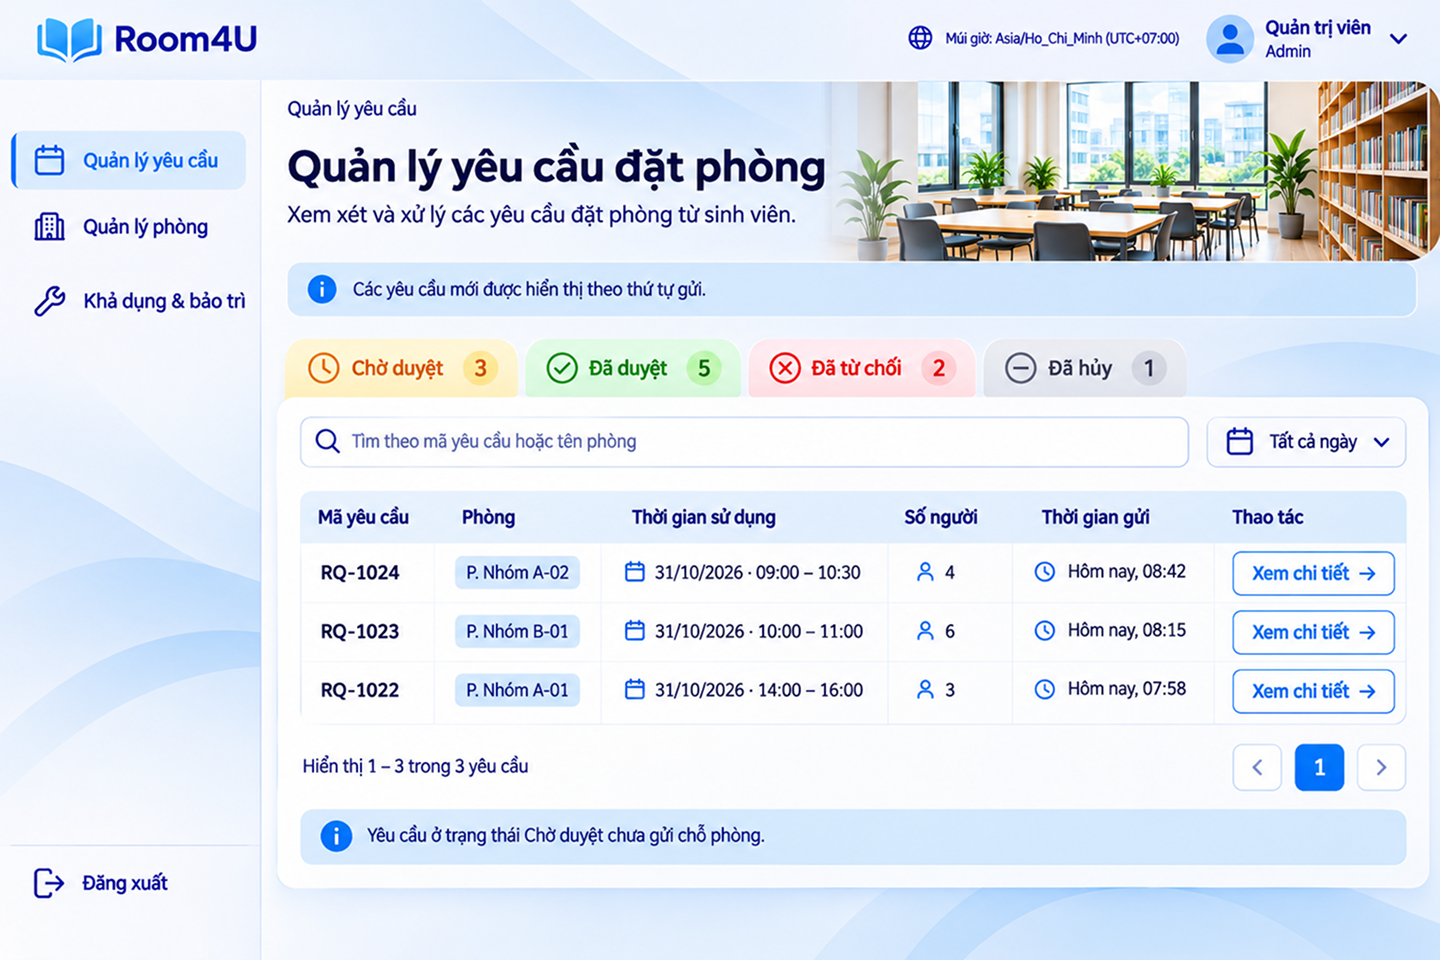
\includegraphics[width=0.9\textwidth,height=0.72\textheight,keepaspectratio]{images/image9.png}
\end{center}

\subsection*{9.2.2.2. S06 - Booking Request Details and
Processing}\label{s06---booking-request-details-and-processing}
\addcontentsline{toc}{subsection}{9.2.2.2. S06 - Booking Request Details
and Processing}

\begin{itemize}
\item
  Description: This screen presents the details and processing controls
  for a selected booking request. Its layout changes according to the
  request status. Common information includes booking details, requester
  information, room information, the room schedule, and
  request-processing history.

  \begin{itemize}
  \item
    Pending Requests: Administrators review the requested date and time,
    duration, number of participants, purpose, notes, requester details,
    room capacity, equipment, and room availability. They can approve a
    request when the slot is valid or reject it by providing a reason.
    Before approval, the system checks for scheduling conflicts. If the
    requested period is no longer available, the interface displays a
    conflict message and does not approve the request.
  \item
    Approved, Rejected, and Cancelled Requests: Administrators can
    review the booking information, current status, processing reason
    when applicable, and request history. For an Approved request, the
    detail screen provides a Cancel Booking action when cancellation is
    permitted. The administrator must enter a reason and confirm the
    action. The cancellation-reason field allows 1--250 characters after
    leading and trailing whitespace are removed (BR-13). Rejected and
    Cancelled requests are presented for review rather than as pending
    requests awaiting approval.
  \end{itemize}
\item
  \textbf{Mockup Views:}
\end{itemize}

\subsubsection{S06.1 -- Pending Request
Details:}\label{s06.1-pending-request-details}

\begin{quote}
\begin{center}
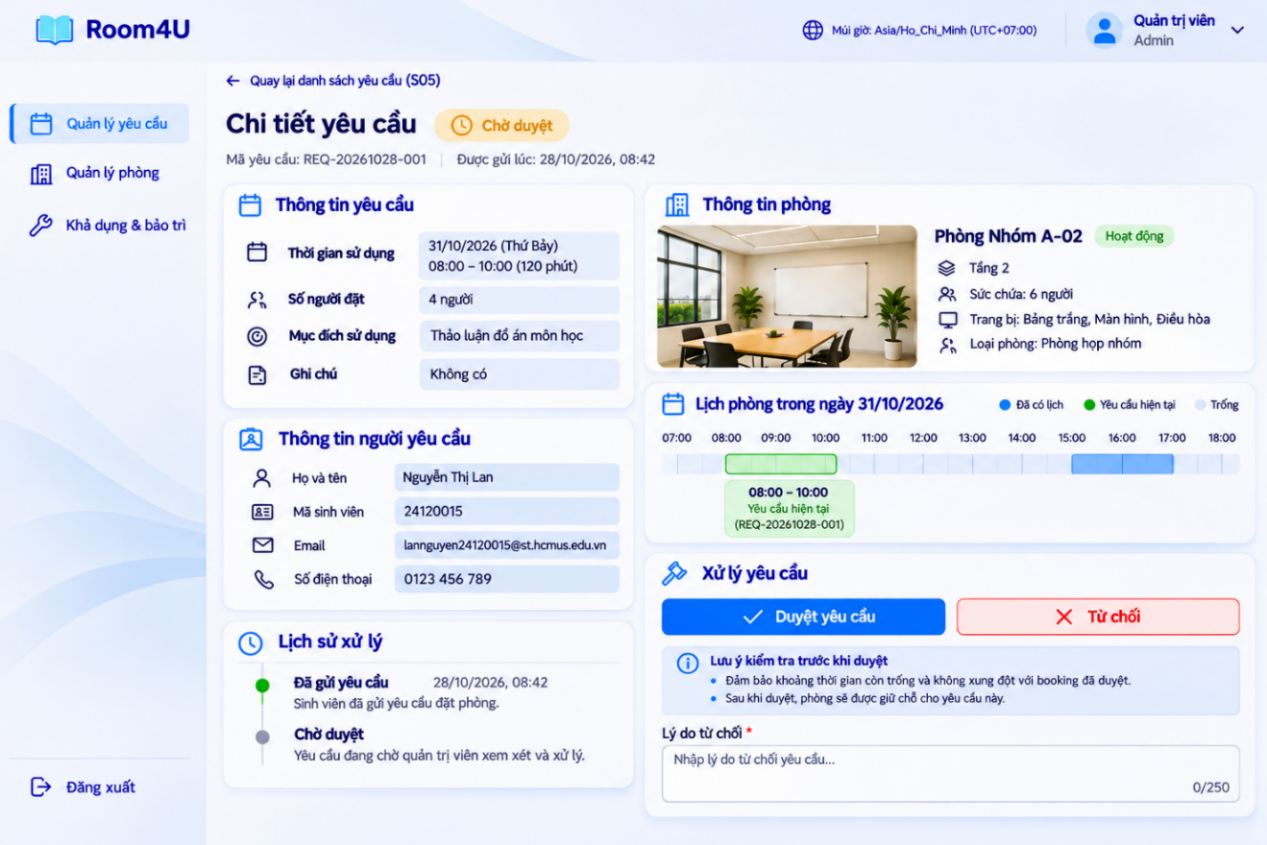
\includegraphics[width=0.9\textwidth,height=0.72\textheight,keepaspectratio]{images/image10.png}
\end{center}
\end{quote}

\subsubsection*{\texorpdfstring{ S06.1a -- Confirm
Approval:}{ S06.1a -- Confirm Approval:}}\label{s06.1a-confirm-approval}
\addcontentsline{toc}{subsubsection}{ S06.1a -- Confirm Approval:}

\begin{quote}
\begin{center}
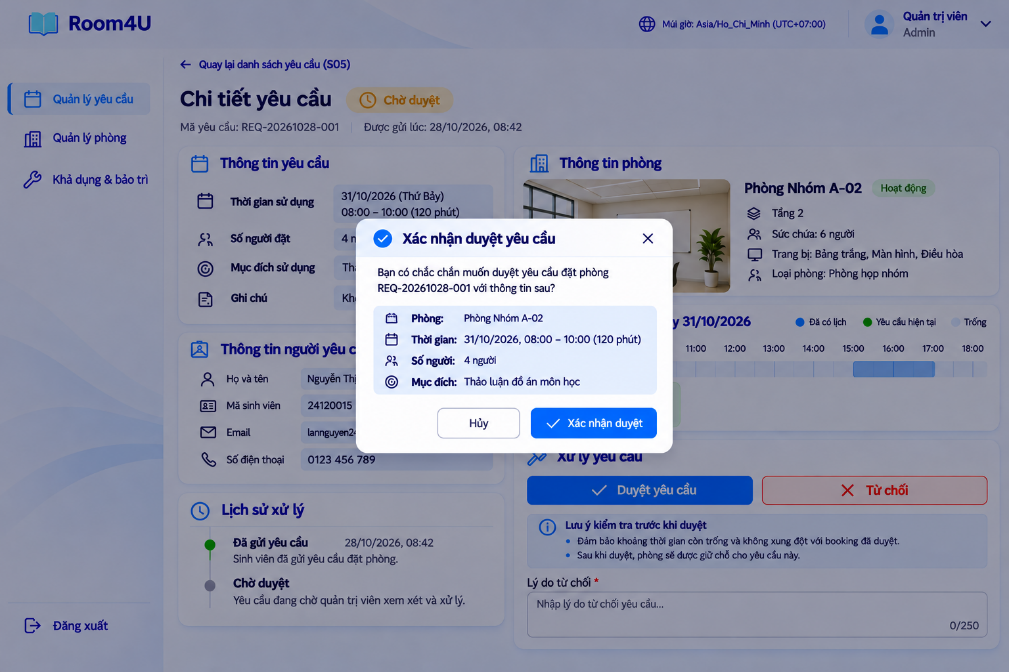
\includegraphics[width=0.9\textwidth,height=0.72\textheight,keepaspectratio]{images/image11.png}
\end{center}
\end{quote}

\subsubsection*{S06.1b -- Reject Request:}\label{s06.1b-reject-request}
\addcontentsline{toc}{subsubsection}{S06.1b -- Reject Request:}

\begin{quote}
\begin{center}
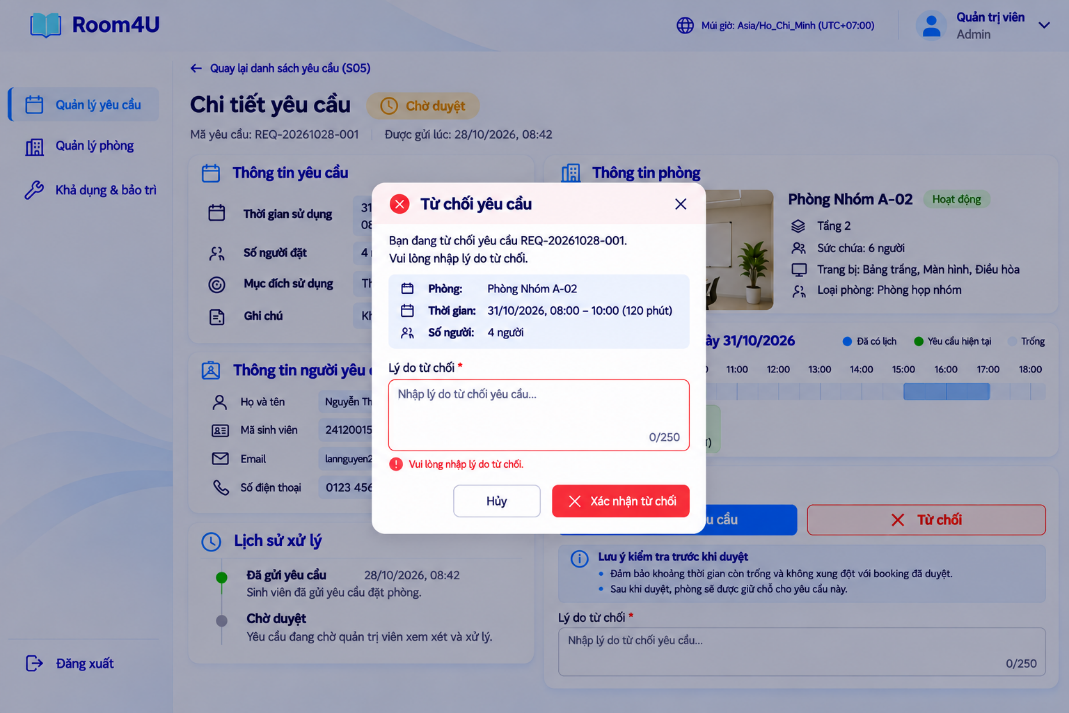
\includegraphics[width=0.9\textwidth,height=0.72\textheight,keepaspectratio]{images/image12.png}
\end{center}
\end{quote}

\subsubsection*{S06.1c -- Approval
Success:}\label{s06.1c-approval-success}
\addcontentsline{toc}{subsubsection}{S06.1c -- Approval Success:}

\begin{quote}
\begin{center}
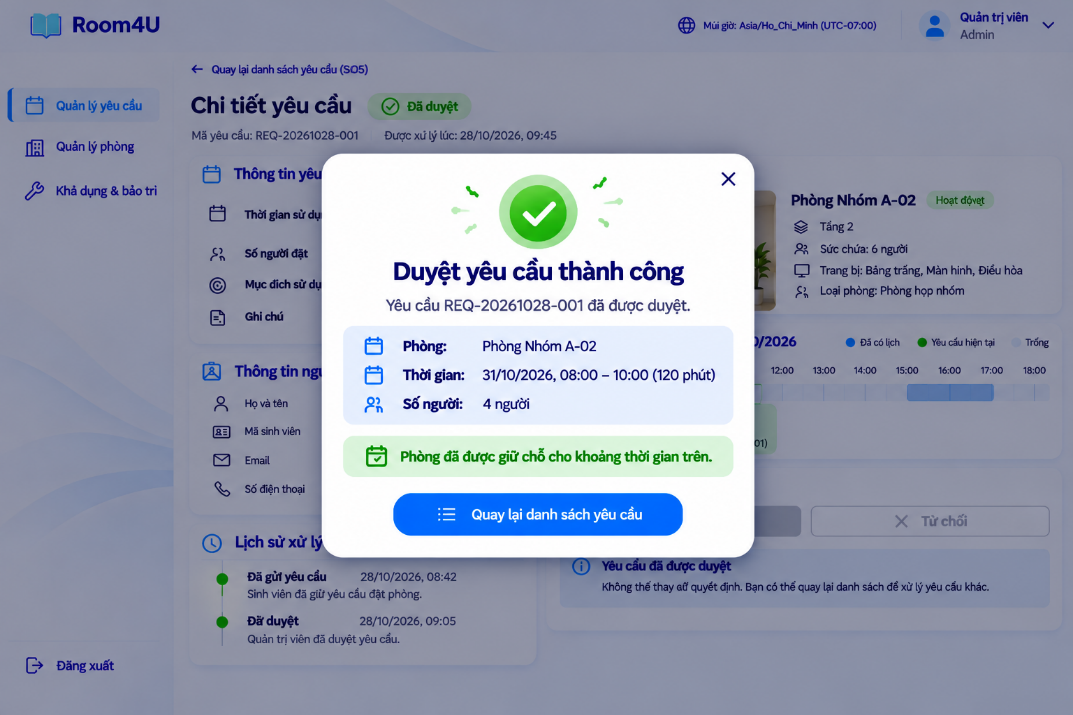
\includegraphics[width=0.9\textwidth,height=0.72\textheight,keepaspectratio]{images/image13.png}
\end{center}
\end{quote}

\subsubsection*{S06.1d -- Rejection
Success:}\label{s06.1d-rejection-success}
\addcontentsline{toc}{subsubsection}{S06.1d -- Rejection Success:}

\begin{quote}
\begin{center}
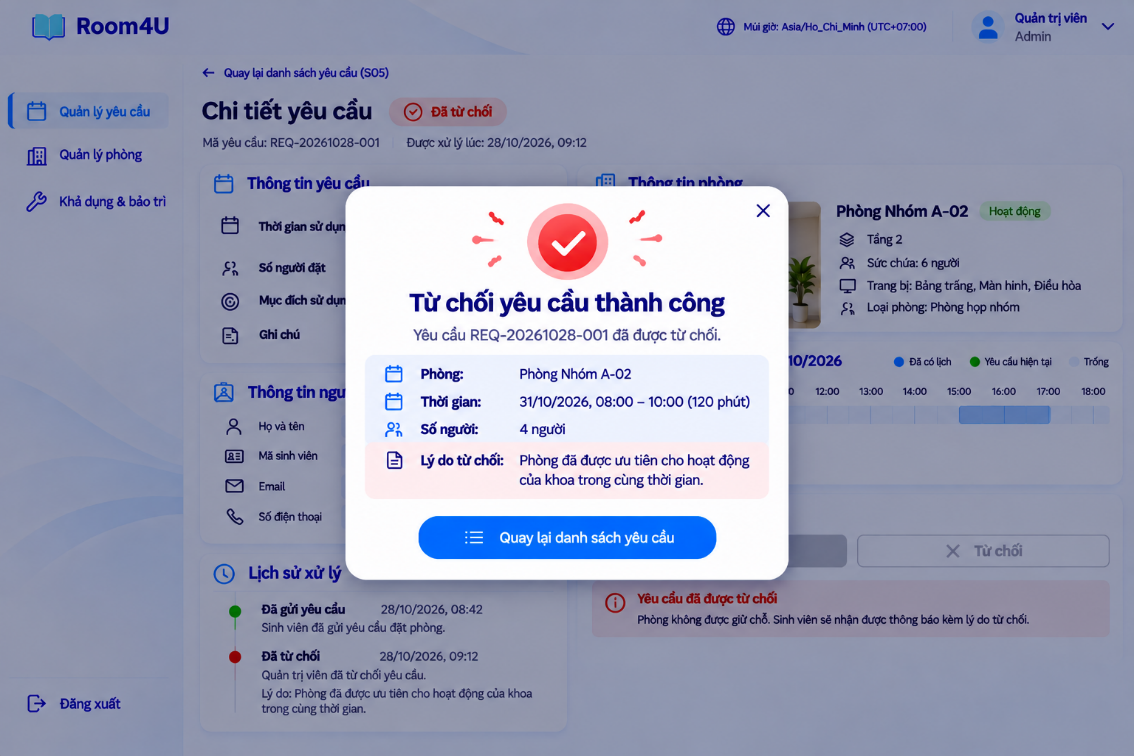
\includegraphics[width=0.9\textwidth,height=0.72\textheight,keepaspectratio]{images/image14.png}
\end{center}
\end{quote}

\subsubsection*{S06.1e -- Scheduling
Conflict:}\label{s06.1e-scheduling-conflict}
\addcontentsline{toc}{subsubsection}{S06.1e -- Scheduling Conflict:}

\begin{quote}
\begin{center}
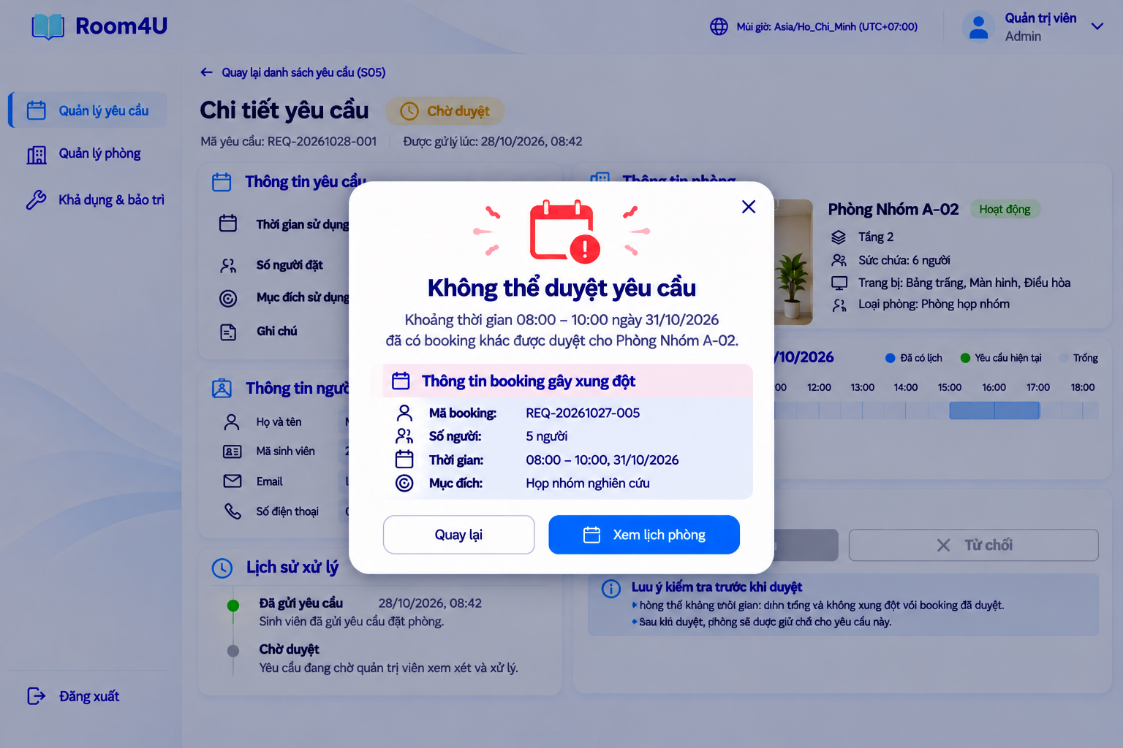
\includegraphics[width=0.9\textwidth,height=0.72\textheight,keepaspectratio]{images/image15.png}
\end{center}
\end{quote}

\subsubsection{S06.2 -- Approved Request Details and
Cancellation:}\label{s06.2-approved-request-details-and-cancellation}

\begin{quote}
\begin{center}
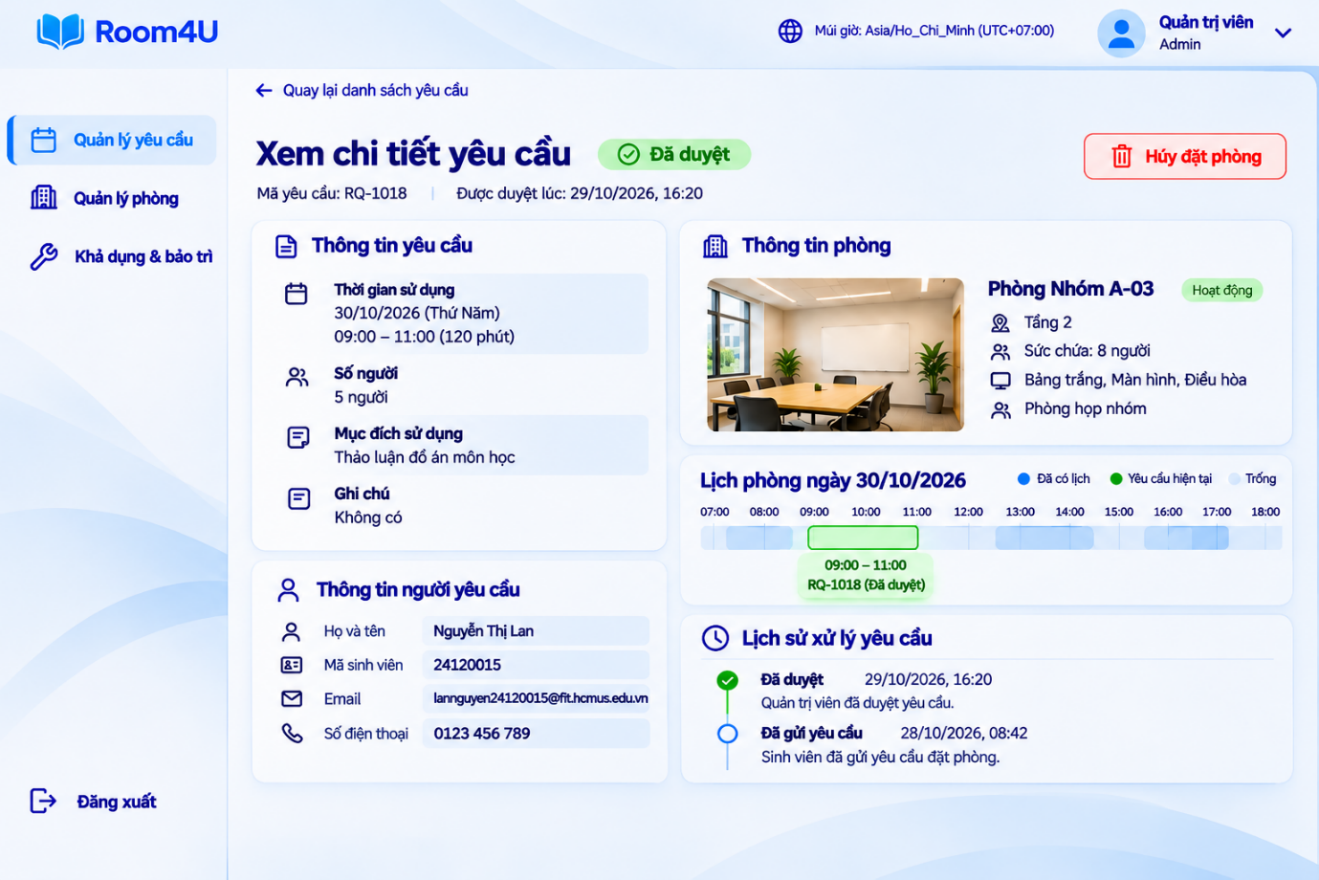
\includegraphics[width=0.9\textwidth,height=0.72\textheight,keepaspectratio]{images/image16.png}
\end{center}

\begin{center}
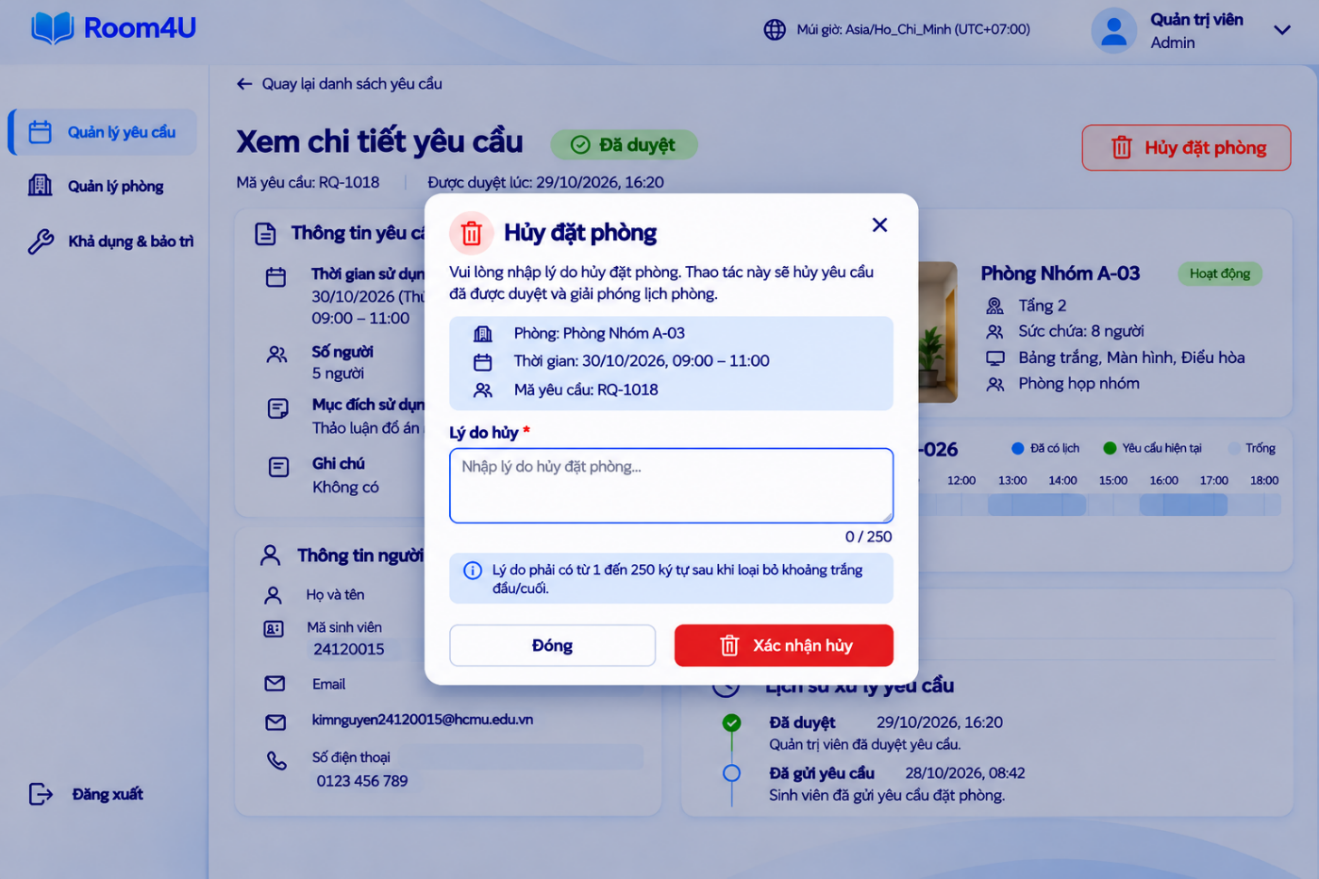
\includegraphics[width=0.9\textwidth,height=0.72\textheight,keepaspectratio]{images/image17.png}
\end{center}

\begin{center}
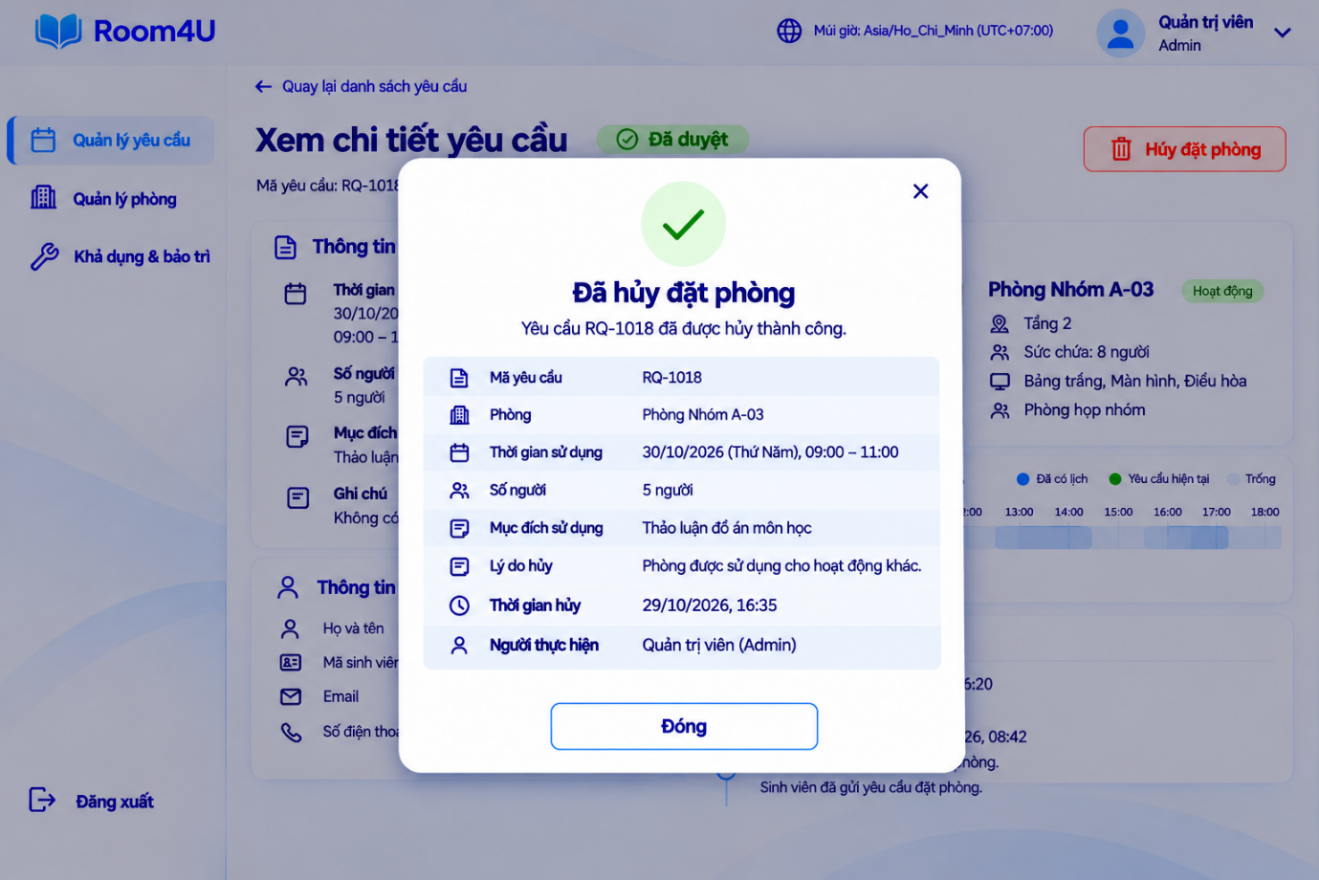
\includegraphics[width=0.9\textwidth,height=0.72\textheight,keepaspectratio]{images/image18.png}
\end{center}
\end{quote}

Approved Booking Cancellation: The administrator can initiate
cancellation from the Approved Request Details screen when the
applicable conditions allow it. A cancellation dialog requests a reason
and asks the administrator to confirm. The reason must contain 1--250
characters after trimming leading and trailing whitespace (BR-13). After
confirmation, the request is updated to Cancelled and the interface
displays the result and relevant booking information.

\subsubsection{S06.3 -- Rejected Request
Details:}\label{s06.3-rejected-request-details}

\begin{quote}
\begin{center}
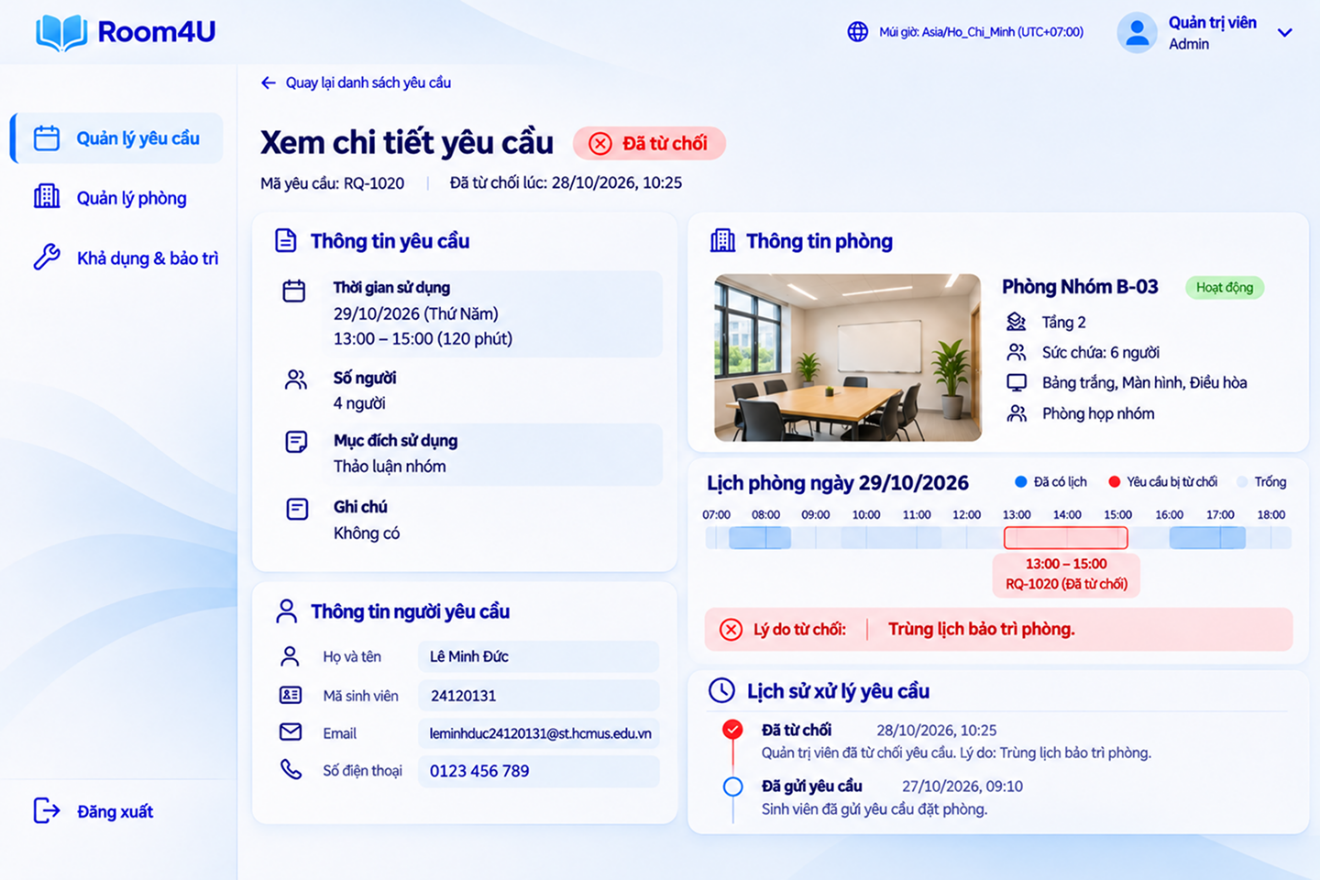
\includegraphics[width=0.9\textwidth,height=0.72\textheight,keepaspectratio]{images/image19.png}
\end{center}
\end{quote}

\subsubsection{S06.4 -- Cancelled Request
Details:}\label{s06.4-cancelled-request-details}

\begin{quote}
\begin{center}
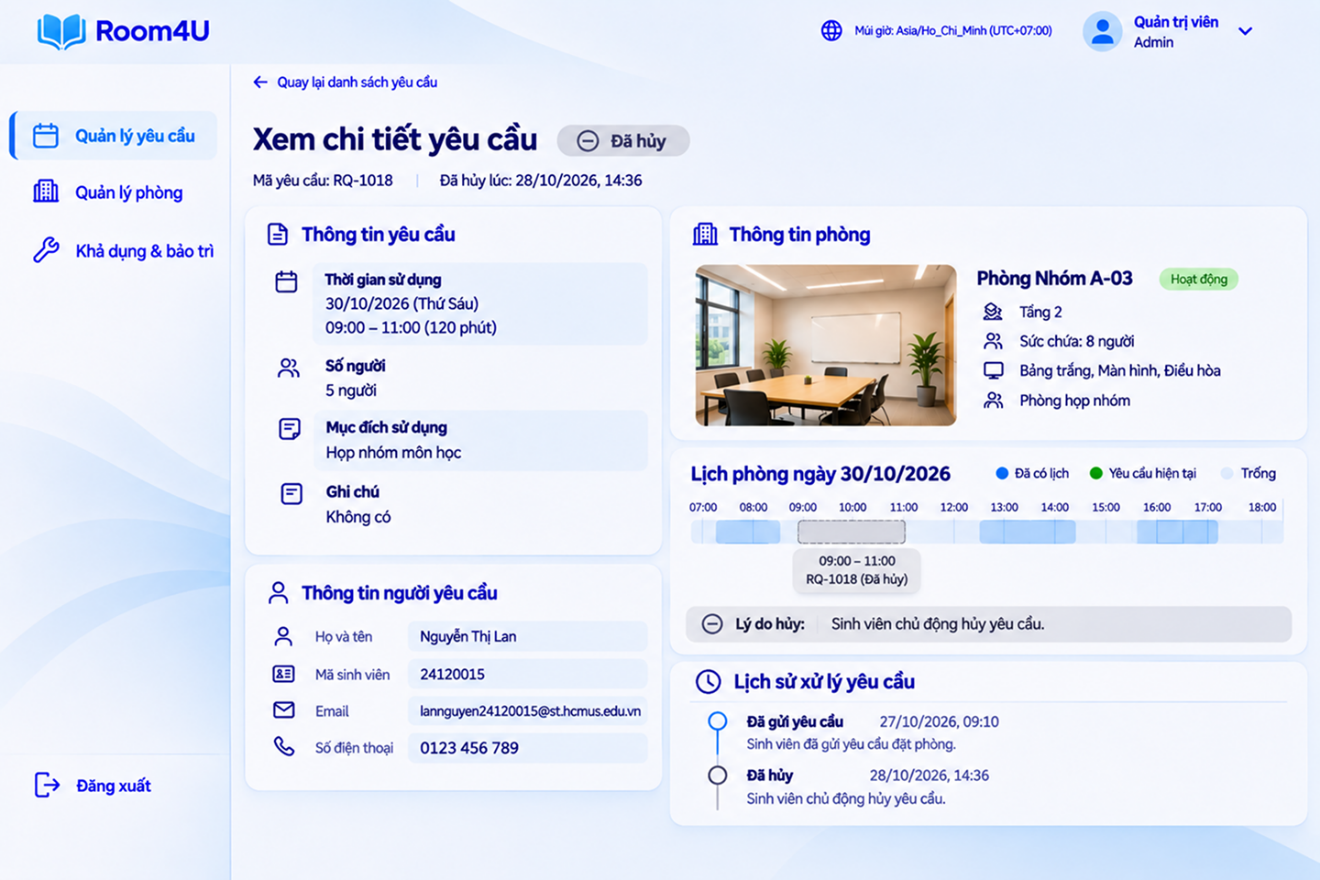
\includegraphics[width=0.9\textwidth,height=0.72\textheight,keepaspectratio]{images/image20.png}
\end{center}
\end{quote}

\subsection*{9.2.2.3. S07 - Room
Management}\label{s07---room-management}
\addcontentsline{toc}{subsection}{9.2.2.3. S07 - Room Management}

\begin{itemize}
\item
  Description: This screen allows administrators to manage room records
  and monitor each room's current status. Summary cards
  show the total number of rooms and the counts of Active, Under
  Maintenance, and Suspended rooms. Administrators can search for a room
  and filter the list by floor or status. The room table and detail
  panel show the room code, room name, floor, capacity, equipment,
  description, and status. Available actions include adding a room,
  editing room information, and suspending or resuming a room, subject
  to the system rules.
\item
  \textbf{Mockup View:}
  \begin{center}
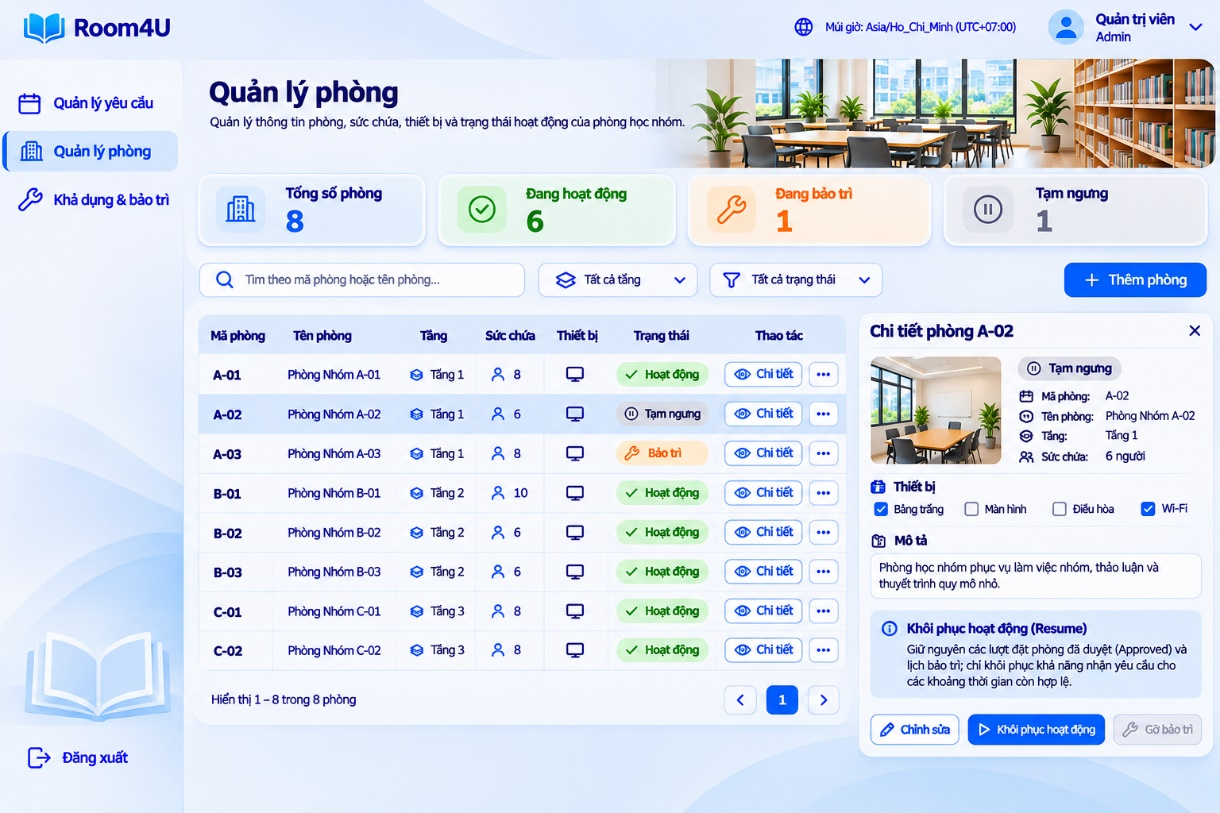
\includegraphics[width=0.9\textwidth,height=0.72\textheight,keepaspectratio]{images/image21.jpeg}
\end{center}
\end{itemize}

Room Creation: The Add Room dialog collects a unique room code, room
name, floor, capacity, equipment selections, and an optional
description. The room code must be unique without case sensitivity after
leading and trailing whitespace are removed. Capacity must be an integer
from 1 to 50. The description is optional and limited to 250 characters.
After a valid submission, a success dialog confirms that the new room
has been added and shows its key details.

Room Editing: The Edit Room dialog displays the selected room's existing
information for update. Administrators can update the room code, name,
floor, capacity, equipment, and optional description. The internal room
ID remains unchanged. The room code may be updated subject to the
uniqueness rules in BR-14. When Save is selected, Room4U revalidates the
fields, including room-code uniqueness, and checks the proposed capacity
against current future Approved bookings. The save is consistent with
concurrent approvals so no future Approved booking can exceed the saved
room capacity. After a valid update, a success dialog confirms that the
room information has been updated.

Suspend and Resume: The room detail panel provides the applicable
room-status action. When a suspended room is resumed, existing Approved
bookings and maintenance schedules are preserved. Resume restores the
ability to receive new booking requests only for time periods that
remain valid; it does not cancel, modify, or overwrite existing bookings
or maintenance records.

\subsection*{9.2.2.4. S08 - Room Availability and
Maintenance}\label{s08---room-availability-and-maintenance}
\addcontentsline{toc}{subsection}{9.2.2.4. S08 - Room Availability and
Maintenance}

\begin{itemize}
\item
  Description: This screen allows administrators to inspect room usage
  and manage maintenance schedules. The interface separates the
  room-usage calendar from the maintenance schedule so that Approved
  bookings and maintenance records can be reviewed without confusing
  their meanings.

  \begin{itemize}
  \item
    Room Usage History: Administrators can inspect room schedules in the
    available calendar views and identify Approved bookings, maintenance
    periods, and available time slots. The schedule is organized by room
    and date to support availability checks.
  \item
    Maintenance Schedule: Administrators can view existing maintenance
    records, create a maintenance schedule, inspect its details, and
    remove its effect when eligible. A maintenance record identifies the
    affected room, start and end time, reason, and status. The
    maintenance list provides view and remove actions; an edit action is
    not included in the current UC-13 flow.
  \item
    Maintenance Rules and Removal Flow: To create a maintenance
    schedule, the administrator specifies the room, start time, end
    time, and reason. The system rejects creation if the requested
    period overlaps an Approved booking or an active maintenance period.
    Creating maintenance does not automatically cancel or modify an
    Approved booking. To remove a schedule's effect, the
    administrator selects a block that is Active and has not started,
    reviews the information, and confirms the action. On success, the
    system removes the block' s effect on availability,
    updates the room schedule, and retains the maintenance record for
    reference. If the block has already started or no longer meets the
    eligibility conditions, the system displays an error and makes no
    change to the record.
  \end{itemize}
\item
  \textbf{Mockup Views:}

  \begin{itemize}
  \item
    \textbf{S08.1 -- Room Usage History:}
  \end{itemize}
\end{itemize}

\begin{quote}
\begin{center}
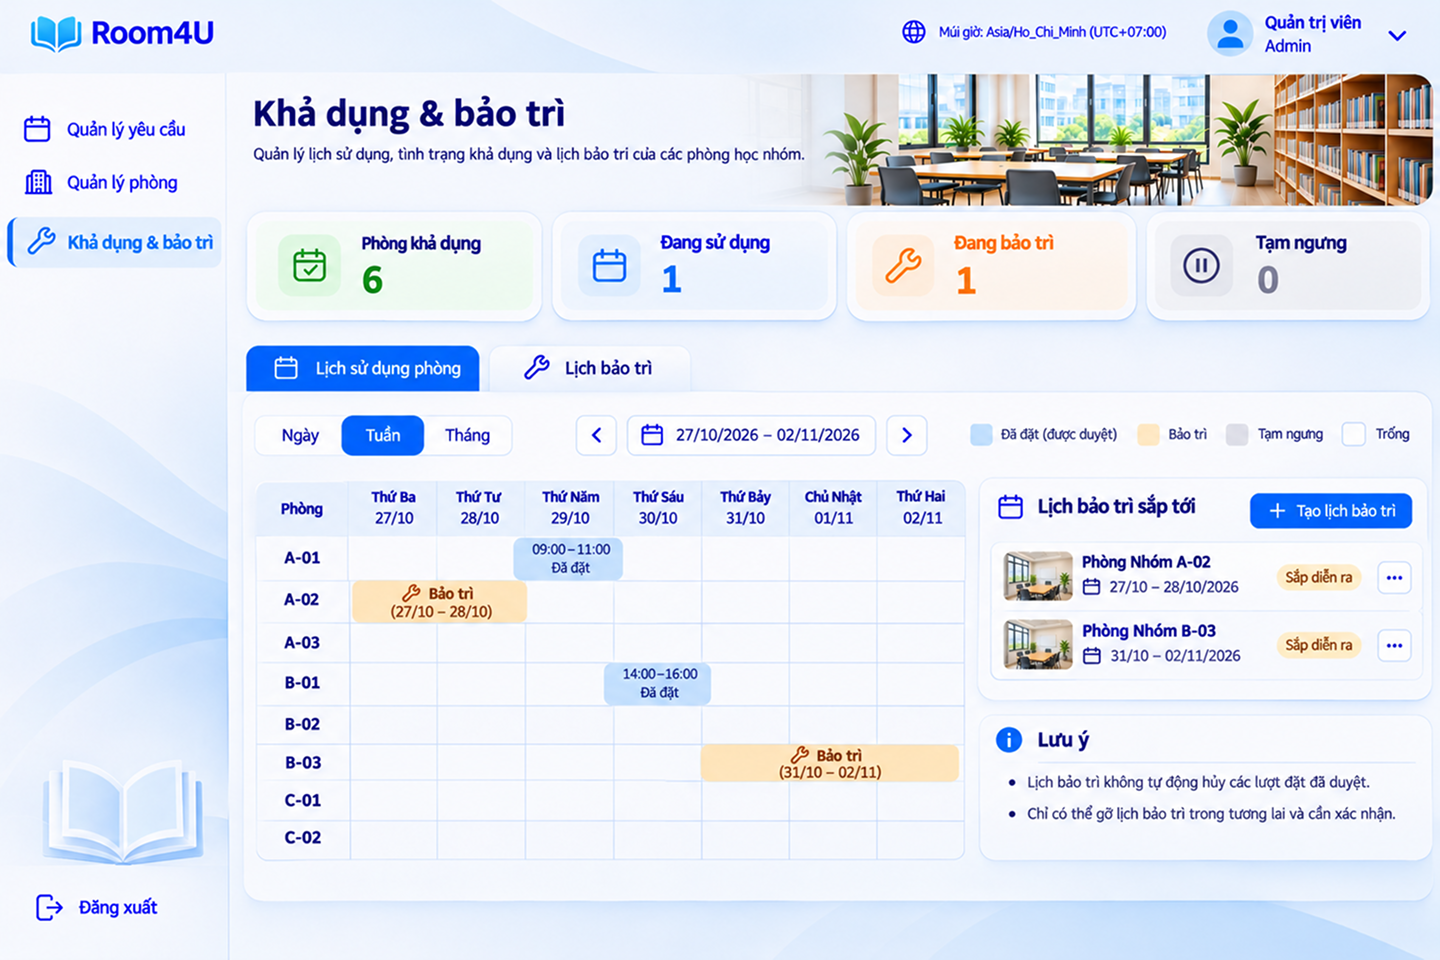
\includegraphics[width=0.9\textwidth,height=0.72\textheight,keepaspectratio]{images/image22.png}
\end{center}
\end{quote}

Create Maintenance Schedule: The creation dialog collects the room,
maintenance date, start time, end time, and reason. The end time must be
later than the start time. The system validates the selected interval
against Approved bookings and active maintenance schedules before
creating the record.

Maintenance List Actions: Each maintenance record can be viewed or
selected for removal when eligible. The current flow does not provide an
edit action. A successful removal deactivates the
schedule's effect but retains its record; unsuccessful
removal leaves the record and schedule unchanged.

\begin{itemize}
\item
  \textbf{S08.2 -- Maintenance Schedule:}
\end{itemize}

\begin{quote}
\begin{center}
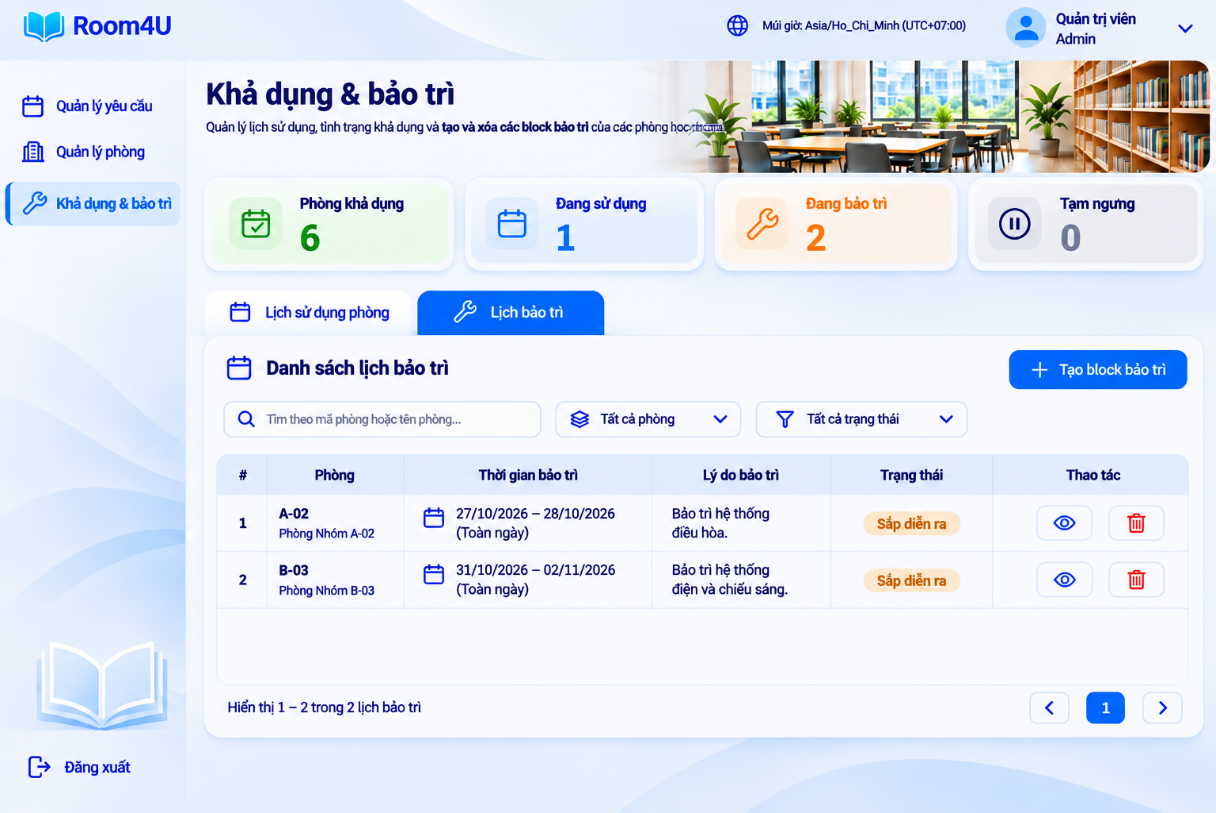
\includegraphics[width=0.9\textwidth,height=0.72\textheight,keepaspectratio]{images/image23.png}
\end{center}

\textbf{Case 1 -- Removal Not Allowed:} The maintenance schedule has
already started. The system explains that the schedule is no longer
eligible for removal, provides the room and schedule details, and offers
a Close action. The record and its effect remain unchanged.

\begin{center}
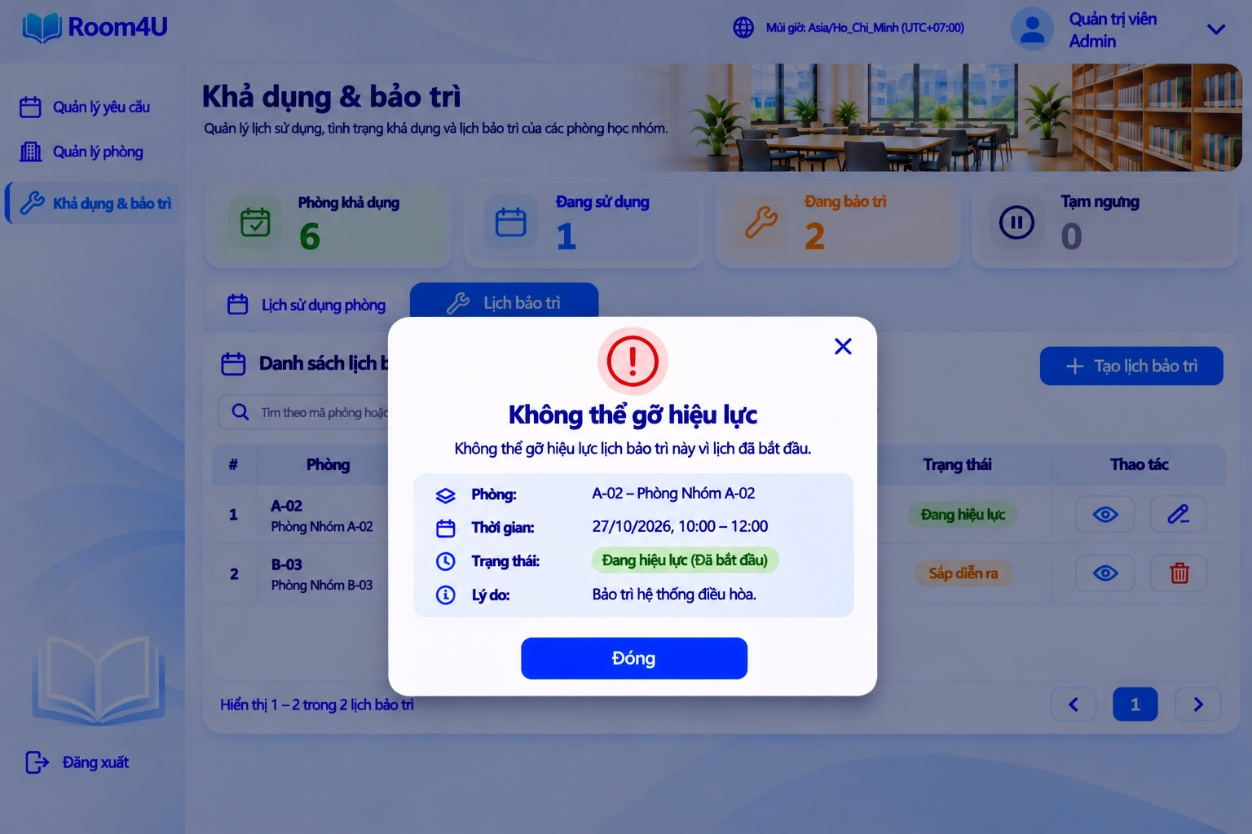
\includegraphics[width=0.9\textwidth,height=0.72\textheight,keepaspectratio]{images/image24.jpeg}
\end{center}

\textbf{Case 2 -- Creation Not Allowed --- Conflicting Approved
Booking:} The system rejects the creation because the requested
maintenance period overlaps with an existing Approved booking (FR-25).
The dialog displays the affected room and conflicting time periods. No
new maintenance record is created, and existing bookings remain
unchanged.

\begin{center}
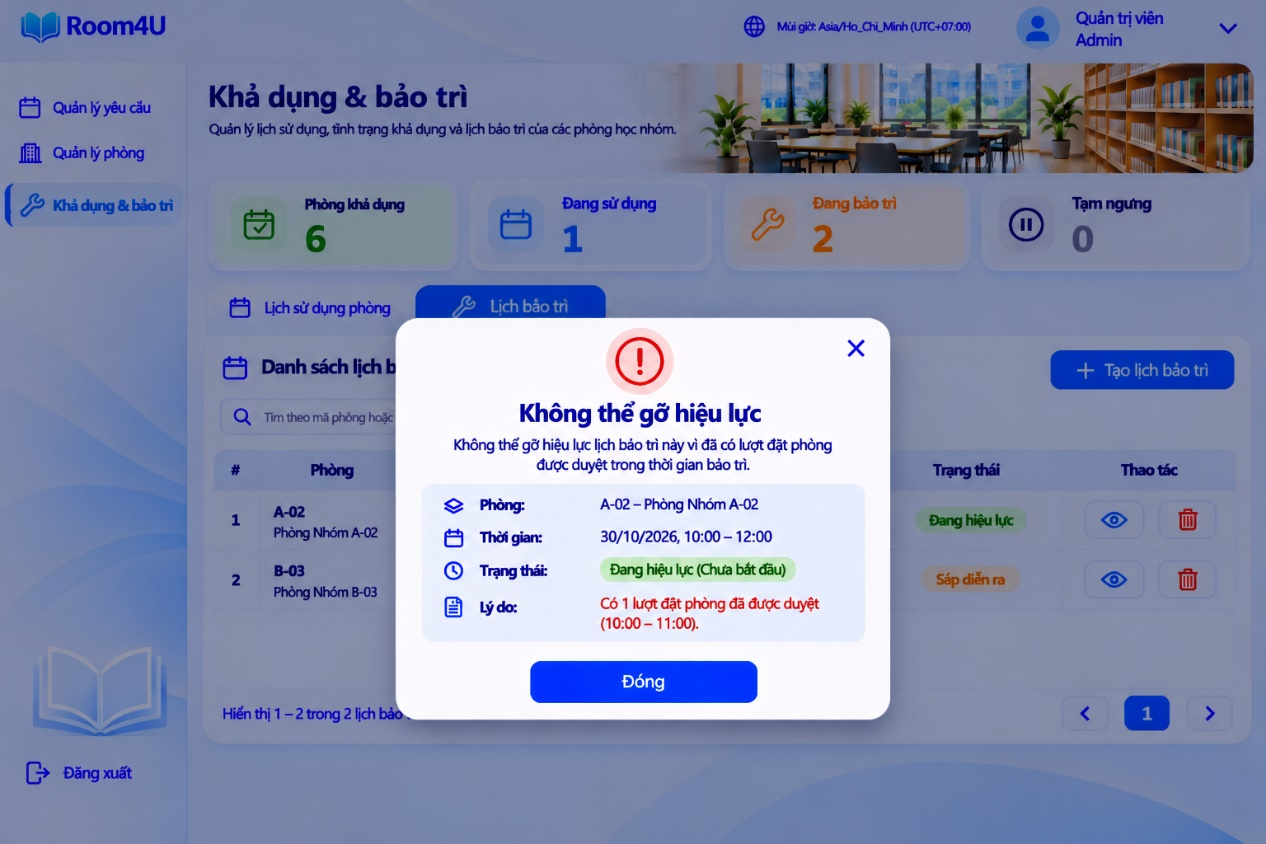
\includegraphics[width=0.9\textwidth,height=0.72\textheight,keepaspectratio]{images/image25.jpeg}
\end{center}
\end{quote}

\section*{9.3. Accessibility
Considerations}\label{accessibility-considerations}
\addcontentsline{toc}{section}{9.3. Accessibility Considerations}

Color and Status Indicators: The blue-and-white palette maintains a
consistent visual hierarchy. Statuses use distinct text labels and
supporting icons as well as color, so meaning is not communicated by
color alone.

Input Labels and Feedback: Form fields use visible labels and helpful
placeholders. Required fields and validation messages should be clearly
identified, especially for booking submission, rejection reasons, room
creation and editing, and administrator cancellation reasons.

\begin{itemize}
\item
  Keyboard and Focus: Interactive controls such as buttons, search
  fields, form inputs, navigation items, and dialogs should have a
  logical keyboard order and a visible focus state during
  implementation.
\item
  Keyboard Navigation: Interactive elements, including buttons, input
  fields, dropdowns, and navigation links, should support keyboard
  navigation to improve accessibility and usability.
\item
  Dialog Feedback: Confirmation, success, and error dialogs should have
  clear titles, concise explanations, and action labels that describe
  the outcome. Error dialogs should explain why an operation is blocked
  and confirm that the underlying record remains unchanged.
\end{itemize}
